% !TEX TS-program = pdflatex
% !TEX encoding = UTF-8 Unicode

% This is a simple template for a LaTeX document using the "article" class.
% See "book", "report", "letter" for other types of document.

\documentclass[11pt]{article} % use larger type; default would be 10pt

\usepackage[utf8]{inputenc} % set input encoding (not needed with XeLaTeX)
\usepackage{graphicx}
\usepackage{listings}
\lstset{language=java,basicstyle=\small}
\usepackage{lscape}
%%% Examples of Article customizations
% These packages are optional, depending whether you want the features they provide.
% See the LaTeX Companion or other references for full information.

%%% PAGE DIMENSIONS
\usepackage{geometry} % to change the page dimensions
\geometry{a4paper} % or letterpaper (US) or a5paper or....
% \geometry{margins=2in} % for example, change the margins to 2 inches all round
% \geometry{landscape} % set up the page for landscape
%   read geometry.pdf for detailed page layout information

\usepackage{graphicx} % support the \includegraphics command and options

% \usepackage[parfill]{parskip} % Activate to begin paragraphs with an empty line rather than an indent

%%% PACKAGES
\usepackage{booktabs} % for much better looking tables
\usepackage{array} % for better arrays (eg matrices) in maths
\usepackage{paralist} % very flexible & customisable lists (eg. enumerate/itemize, etc.)
\usepackage{verbatim} % adds environment for commenting out blocks of text & for better verbatim
\usepackage{subfig} % make it possible to include more than one captioned figure/table in a single float
% These packages are all incorporated in the memoir class to one degree or another...

%%% HEADERS & FOOTERS
\usepackage{fancyhdr} % This should be set AFTER setting up the page geometry
\pagestyle{fancy} % options: empty , plain , fancy
\renewcommand{\headrulewidth}{0pt} % customise the layout...
\lhead{}\chead{}\rhead{}
\lfoot{}\cfoot{\thepage}\rfoot{}

%%% SECTION TITLE APPEARANCE
\usepackage{sectsty}
\allsectionsfont{\sffamily\mdseries\upshape} % (See the fntguide.pdf for font help)
% (This matches ConTeXt defaults)

%%% ToC (table of contents) APPEARANCE
\usepackage[nottoc,notlof,notlot]{tocbibind} % Put the bibliography in the ToC
\usepackage[titles,subfigure]{tocloft} % Alter the style of the Table of Contents
\renewcommand{\cftsecfont}{\rmfamily\mdseries\upshape}
\renewcommand{\cftsecpagefont}{\rmfamily\mdseries\upshape} % No bold!

%%% END Article customizations

%%% The "real" document content comes below...

\title{Phone E-Checkout App}
\author{Hans Dulimarta}
\date{\texttt{dulimarh@cis.gvsu.edu}}
%\date{} % Activate to display a given date or no date (if empty),
         % otherwise the current date is printed 

\begin{document}
\landscape
\maketitle

\section{Introduction}
The Phone E-Checkout program consists of two separate apps.
\begin{itemize}
\item \texttt{DeviceQR} that runs on the phone being checked out by a student
\item \texttt{PhoneCheckout} that runs on the instructor's phone. The
first screen of this app lists all the phones currently checked out
(PhoneID + student userid)
\end{itemize}

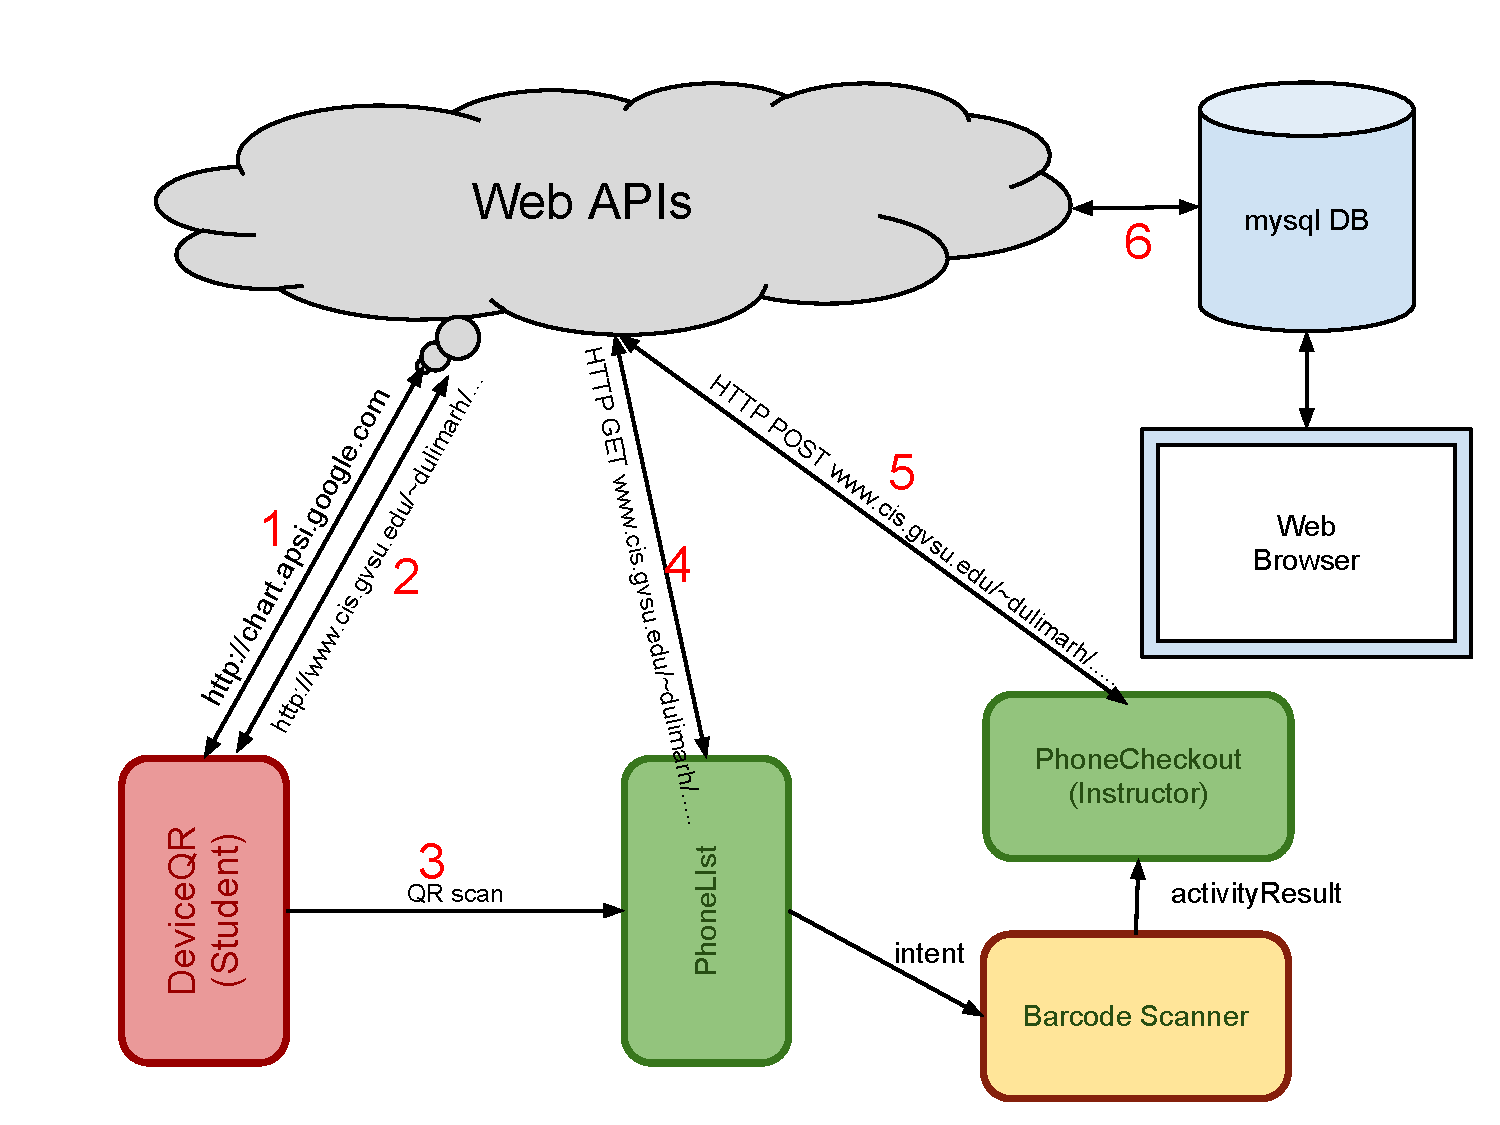
\includegraphics[width=5in]{PhoneCheckout}

\begin{enumerate}
\item Using Android TelephonyManager service, \texttt{DeviceQR}
obtains the phone DeviceID and shows it using a QR Code generated from
http://chart.apis.google.com/chart. This HTTP GET request runs inside
an AsyncTask (\texttt{URLTask}).
\lstinputlisting[firstline=91,lastline=94]{IMEI2QRActivity.java}

\item Using the same AsyncTask, \texttt{DeviceQR} checks if the device
was checked out. It makes another HTTP GET to
http://.../checkout.php?device=xyz and receives a JSON output that
includes the device id, the user id, name of the student who checked
the phone out, and timestamp of checkout. This information is produced
by PHP script that runs queries to a MySQL database running on the EOS
server.
\lstinputlisting[firstline=96,lastline=104]{IMEI2QRActivity.java}

\item To initiate e-checkout, the \texttt{PhoneCheckout} app 
on the instructor's phone scans the QR code with the BarCode Scanner
app (invoked via an Intent). 
\lstinputlisting[firstline=80,lastline=86]{PhoneListActivity.java}

The PhoneID string returned by the
BarCode Scanner is then checked using another HTTP GET to query the
database.
\lstinputlisting[firstline=60,lastline=71]{PhoneListActivity.java}

\item During the e-checkout transaction, the student signs his/her
name on screen prior to confirming the transcaction.
\item To record the transaction, an HTTP POST is issued and the
phoneID, user name, userid, time of checkout, and student signature
are recorded in the database.
\lstinputlisting[firstline=104,lastline=115]{PhoneCheckoutActivity.java}
\item All the HTTP GET and POST requests are translated to mysql SELECT and
   INSERT queries
\end{enumerate}

\section{HTTP POST}
When you submit a form on a web browser, the data in the form are transmitted
to the server using HTTP POST. To send multiple data items to the server
HTTP POST relies on MIME (Multipurpose Internet Mail Extension) encoding.
This is exactly the same encoding technique used for sending 
(multiple) attachments in an email.

The code snippet above posts four different "attachments" (name, device,
time, and image). \texttt{MultipartEntity}, \texttt{StringBody},
\texttt{FileBody} are classes from an additional library included
in the project (\texttt{httpmime-4.1.3.jar}).

\section{SignatureView}
The signature box is a customized View designed to handle the user scribbles 
on the screen. The design of this class is mainly based on the \texttt{FingerPaint}
example found under the APIDemos in the SDK sample. Additional logic was
added to the original FingerPaint example to handle dots in the scribble.
The main technique used to capture the signature is 
to override the \texttt{onTouchEvent} method. Several factors that determines
the design of the \texttt{SignatureView} class:
\begin{enumerate}
\item A signature may consist of several strokes.
\item A single stroke begins when the user's finger tip touches the screen
  (\verb+ACTION_DOWN+),
   and ends when the finger tip leaves the screen (\verb+ACTION_UP+).
   In between these two events the finger tip moves across the screen
   (\verb+ACTION_MOVE+).
\end{enumerate}

\begin{center}
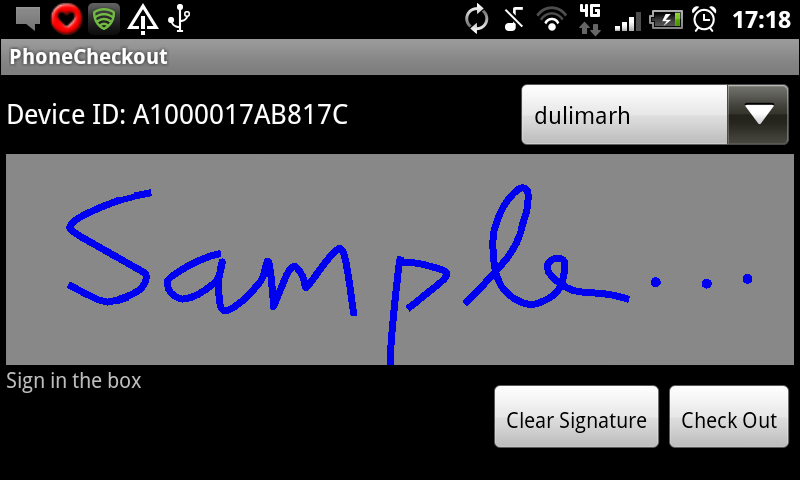
\includegraphics[width=6in]{signature}
\end{center}

To record a signature with multiple strokes:
\begin{itemize}
\item Each stroke is recorded in a \texttt{Path}. 
\item At the beginning of
   a signature stroke the path is reset and the starting coordinate
   of the stroke is recorded.
   \lstinputlisting[firstline=88,lastline=89,numbers=none]{SignatureView.java}
\item At the end of a stroke the path is drawn to a canvas.
    \lstinputlisting[firstline=105,lastline=113,numbers=none]{SignatureView.java}
\item As the finger tip scribles a stroke, bezier curves are added to the 
    path.
    \lstinputlisting[firstline=98,lastline=99,numbers=none]{SignatureView.java}
\item While the \texttt{onTouch()} method records the fingertip motions
   the \texttt{onDraw()} methods renders the signature using the
   following technique:
   \begin{itemize}
   \item The current stroke is rendered from the path
   \item The previously recorded strokes are rendered from the canvas
   \end{itemize}
\end{itemize}

\section{Downloading The Source Code}
The source code of these two apps are available for download from the CIS git repository.
Use the following URI:

\begin{center}
\texttt{cis163@eos08.cis.gvsu.edu:PhoneCheckout.git}
\end{center}
[You can always replace eos08 with any other eosxx hostname]
\end{document}
